\documentclass[1p]{elsarticle_modified}
%\bibliographystyle{elsarticle-num}

%\usepackage[colorlinks]{hyperref}
%\usepackage{abbrmath_seonhwa} %\Abb, \Ascr, \Acal ,\Abf, \Afrak
\usepackage{amsfonts}
\usepackage{amssymb}
\usepackage{amsmath}
\usepackage{amsthm}
\usepackage{scalefnt}
\usepackage{amsbsy}
\usepackage{kotex}
\usepackage{caption}
\usepackage{subfig}
\usepackage{color}
\usepackage{graphicx}
\usepackage{xcolor} %% white, black, red, green, blue, cyan, magenta, yellow
\usepackage{float}
\usepackage{setspace}
\usepackage{hyperref}

\usepackage{tikz}
\usetikzlibrary{arrows}

\usepackage{multirow}
\usepackage{array} % fixed length table
\usepackage{hhline}

%%%%%%%%%%%%%%%%%%%%%
\makeatletter
\renewcommand*\env@matrix[1][\arraystretch]{%
	\edef\arraystretch{#1}%
	\hskip -\arraycolsep
	\let\@ifnextchar\new@ifnextchar
	\array{*\c@MaxMatrixCols c}}
\makeatother %https://tex.stackexchange.com/questions/14071/how-can-i-increase-the-line-spacing-in-a-matrix
%%%%%%%%%%%%%%%

\usepackage[normalem]{ulem}

\newcommand{\msout}[1]{\ifmmode\text{\sout{\ensuremath{#1}}}\else\sout{#1}\fi}
%SOURCE: \msout is \stkout macro in https://tex.stackexchange.com/questions/20609/strikeout-in-math-mode

\newcommand{\cancel}[1]{
	\ifmmode
	{\color{red}\msout{#1}}
	\else
	{\color{red}\sout{#1}}
	\fi
}

\newcommand{\add}[1]{
	{\color{blue}\uwave{#1}}
}

\newcommand{\replace}[2]{
	\ifmmode
	{\color{red}\msout{#1}}{\color{blue}\uwave{#2}}
	\else
	{\color{red}\sout{#1}}{\color{blue}\uwave{#2}}
	\fi
}

\newcommand{\Sol}{\mathcal{S}} %segment
\newcommand{\D}{D} %diagram
\newcommand{\A}{\mathcal{A}} %arc


%%%%%%%%%%%%%%%%%%%%%%%%%%%%%5 test

\def\sl{\operatorname{\textup{SL}}(2,\Cbb)}
\def\psl{\operatorname{\textup{PSL}}(2,\Cbb)}
\def\quan{\mkern 1mu \triangleright \mkern 1mu}

\theoremstyle{definition}
\newtheorem{thm}{Theorem}[section]
\newtheorem{prop}[thm]{Proposition}
\newtheorem{lem}[thm]{Lemma}
\newtheorem{ques}[thm]{Question}
\newtheorem{cor}[thm]{Corollary}
\newtheorem{defn}[thm]{Definition}
\newtheorem{exam}[thm]{Example}
\newtheorem{rmk}[thm]{Remark}
\newtheorem{alg}[thm]{Algorithm}

\newcommand{\I}{\sqrt{-1}}
\begin{document}

%\begin{frontmatter}
%
%\title{Boundary parabolic representations of knots up to 8 crossings}
%
%%% Group authors per affiliation:
%\author{Yunhi Cho} 
%\address{Department of Mathematics, University of Seoul, Seoul, Korea}
%\ead{yhcho@uos.ac.kr}
%
%
%\author{Seonhwa Kim} %\fnref{s_kim}}
%\address{Center for Geometry and Physics, Institute for Basic Science, Pohang, 37673, Korea}
%\ead{ryeona17@ibs.re.kr}
%
%\author{Hyuk Kim}
%\address{Department of Mathematical Sciences, Seoul National University, Seoul 08826, Korea}
%\ead{hyukkim@snu.ac.kr}
%
%\author{Seokbeom Yoon}
%\address{Department of Mathematical Sciences, Seoul National University, Seoul, 08826,  Korea}
%\ead{sbyoon15@snu.ac.kr}
%
%\begin{abstract}
%We find all boundary parabolic representation of knots up to 8 crossings.
%
%\end{abstract}
%\begin{keyword}
%    \MSC[2010] 57M25 
%\end{keyword}
%
%\end{frontmatter}

%\linenumbers
%\tableofcontents
%
\newcommand\colored[1]{\textcolor{white}{\rule[-0.35ex]{0.8em}{1.4ex}}\kern-0.8em\color{red} #1}%
%\newcommand\colored[1]{\textcolor{white}{ #1}\kern-2.17ex	\textcolor{white}{ #1}\kern-1.81ex	\textcolor{white}{ #1}\kern-2.15ex\color{red}#1	}

{\Large $\underline{11a_{198}~(K11a_{198})}$}

\setlength{\tabcolsep}{10pt}
\renewcommand{\arraystretch}{1.6}
\vspace{1cm}\begin{tabular}{m{100pt}>{\centering\arraybackslash}m{274pt}}
\multirow{5}{120pt}{
	\centering
	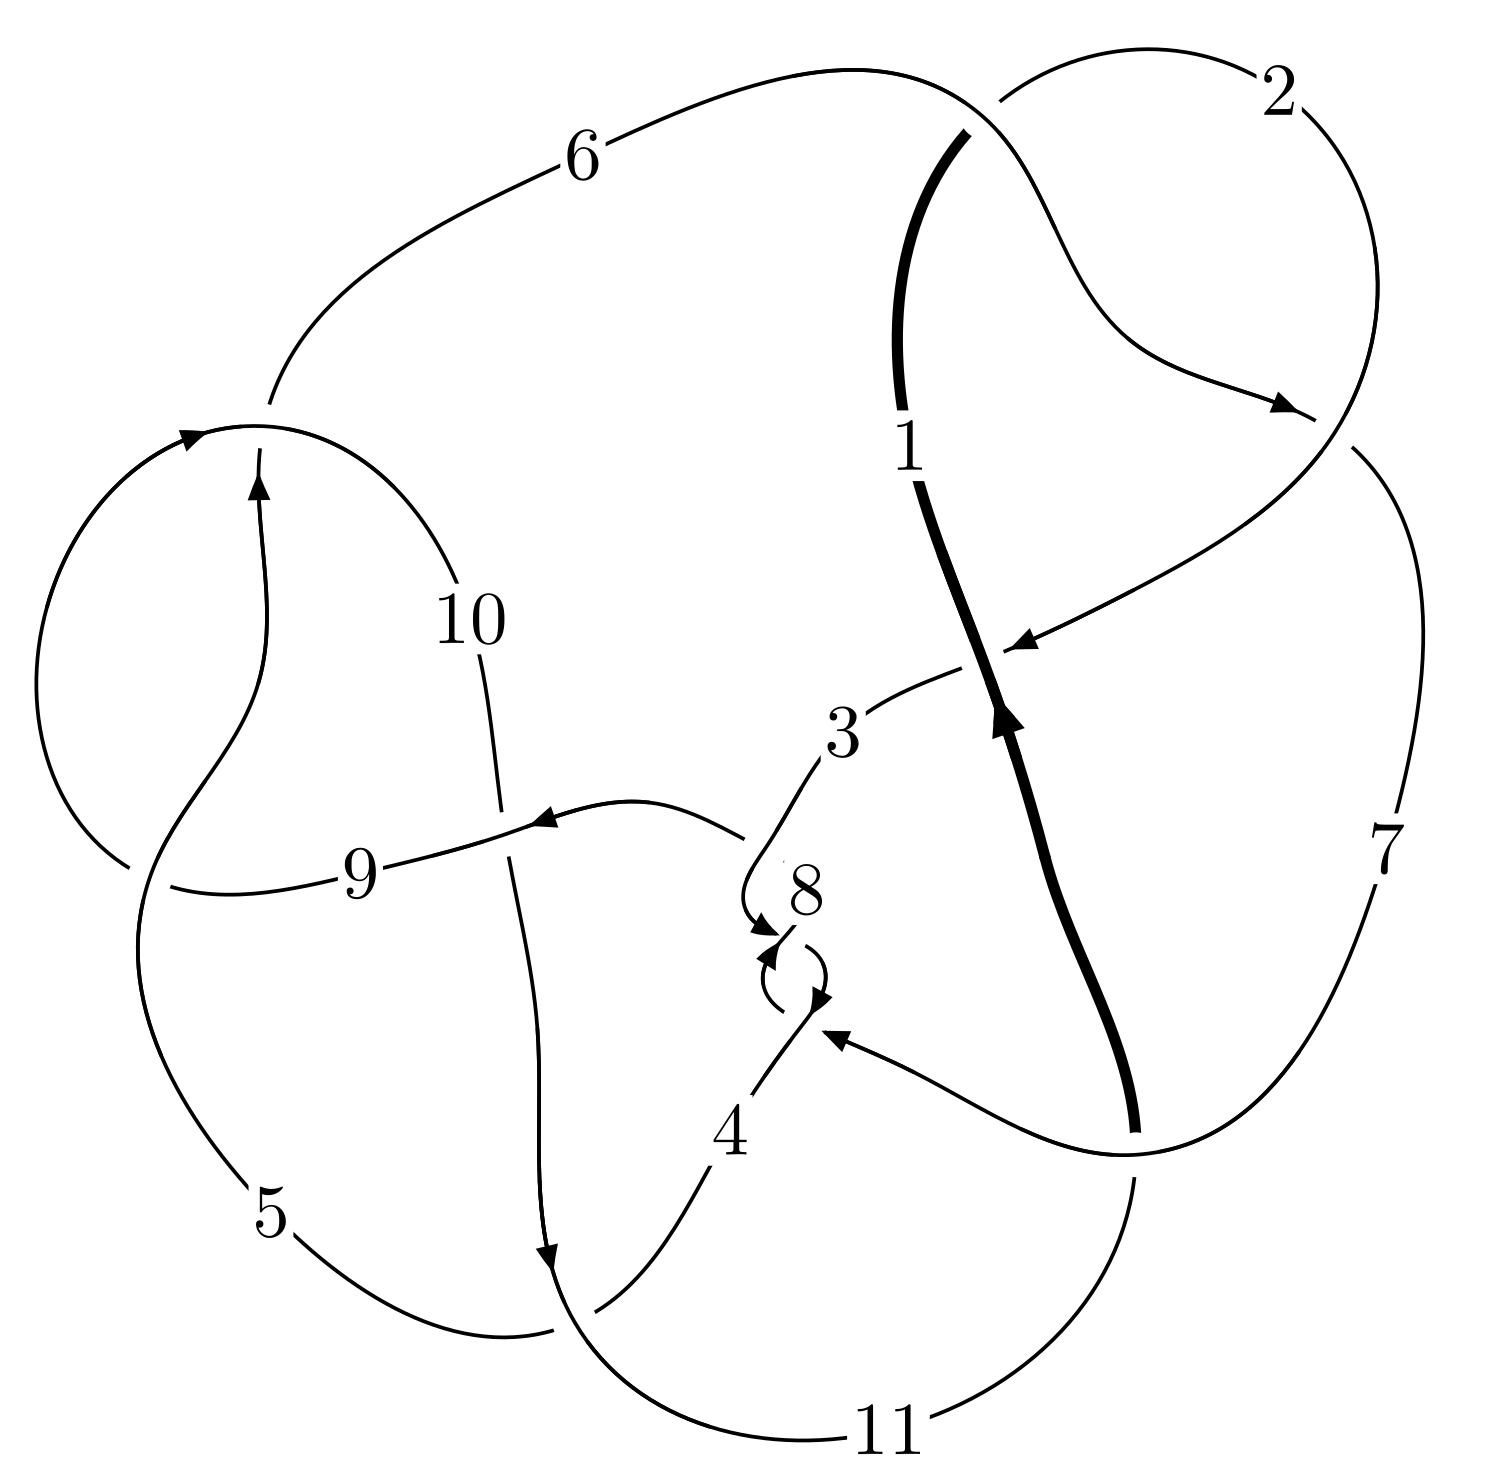
\includegraphics[width=112pt]{../../../GIT/diagram.site/Diagrams/png/447_11a_198.png}\\
\ \ \ A knot diagram\footnotemark}&
\allowdisplaybreaks
\textbf{Linearized knot diagam} \\
\cline{2-2}
 &
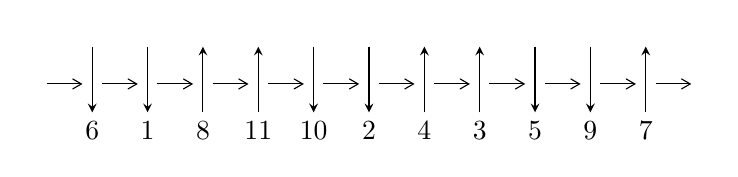
\begin{tikzpicture}[x=20pt, y=17pt]
	% nodes
	\node (C0) at (0, 0) {};
	\node (C1) at (1, 0) {};
	\node (C1U) at (1, +1) {};
	\node (C1D) at (1, -1) {6};

	\node (C2) at (2, 0) {};
	\node (C2U) at (2, +1) {};
	\node (C2D) at (2, -1) {1};

	\node (C3) at (3, 0) {};
	\node (C3U) at (3, +1) {};
	\node (C3D) at (3, -1) {8};

	\node (C4) at (4, 0) {};
	\node (C4U) at (4, +1) {};
	\node (C4D) at (4, -1) {11};

	\node (C5) at (5, 0) {};
	\node (C5U) at (5, +1) {};
	\node (C5D) at (5, -1) {10};

	\node (C6) at (6, 0) {};
	\node (C6U) at (6, +1) {};
	\node (C6D) at (6, -1) {2};

	\node (C7) at (7, 0) {};
	\node (C7U) at (7, +1) {};
	\node (C7D) at (7, -1) {4};

	\node (C8) at (8, 0) {};
	\node (C8U) at (8, +1) {};
	\node (C8D) at (8, -1) {3};

	\node (C9) at (9, 0) {};
	\node (C9U) at (9, +1) {};
	\node (C9D) at (9, -1) {5};

	\node (C10) at (10, 0) {};
	\node (C10U) at (10, +1) {};
	\node (C10D) at (10, -1) {9};

	\node (C11) at (11, 0) {};
	\node (C11U) at (11, +1) {};
	\node (C11D) at (11, -1) {7};
	\node (C12) at (12, 0) {};

	% arrows
	\draw[->,>={angle 60}]
	(C0) edge (C1) (C1) edge (C2) (C2) edge (C3) (C3) edge (C4) (C4) edge (C5) (C5) edge (C6) (C6) edge (C7) (C7) edge (C8) (C8) edge (C9) (C9) edge (C10) (C10) edge (C11) (C11) edge (C12) ;	\draw[->,>=stealth]
	(C1U) edge (C1D) (C2U) edge (C2D) (C3D) edge (C3U) (C4D) edge (C4U) (C5U) edge (C5D) (C6U) edge (C6D) (C7D) edge (C7U) (C8D) edge (C8U) (C9U) edge (C9D) (C10U) edge (C10D) (C11D) edge (C11U) ;
	\end{tikzpicture} \\
\hhline{~~} \\& 
\textbf{Solving Sequence} \\ \cline{2-2} 
 &
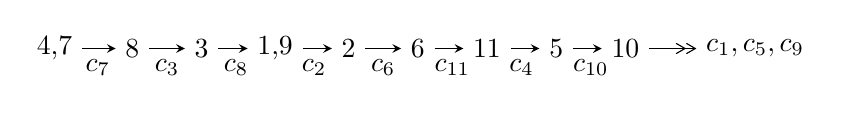
\begin{tikzpicture}[x=25pt, y=7pt]
	% node
	\node (A0) at (-1/8, 0) {4,7};
	\node (A1) at (1, 0) {8};
	\node (A2) at (2, 0) {3};
	\node (A3) at (49/16, 0) {1,9};
	\node (A4) at (33/8, 0) {2};
	\node (A5) at (41/8, 0) {6};
	\node (A6) at (49/8, 0) {11};
	\node (A7) at (57/8, 0) {5};
	\node (A8) at (65/8, 0) {10};
	\node (C1) at (1/2, -1) {$c_{7}$};
	\node (C2) at (3/2, -1) {$c_{3}$};
	\node (C3) at (5/2, -1) {$c_{8}$};
	\node (C4) at (29/8, -1) {$c_{2}$};
	\node (C5) at (37/8, -1) {$c_{6}$};
	\node (C6) at (45/8, -1) {$c_{11}$};
	\node (C7) at (53/8, -1) {$c_{4}$};
	\node (C8) at (61/8, -1) {$c_{10}$};
	\node (A9) at (10, 0) {$c_{1},c_{5},c_{9}$};

	% edge
	\draw[->,>=stealth]	
	(A0) edge (A1) (A1) edge (A2) (A2) edge (A3) (A3) edge (A4) (A4) edge (A5) (A5) edge (A6) (A6) edge (A7) (A7) edge (A8) ;
	\draw[->>,>={angle 60}]	
	(A8) edge (A9);
\end{tikzpicture} \\ 

\end{tabular} \\

\footnotetext{
The image of knot diagram is generated by the software ``\textbf{Draw programme}" developed by Andrew Bartholomew(\url{http://www.layer8.co.uk/maths/draw/index.htm\#Running-draw}), where we modified some parts for our purpose(\url{https://github.com/CATsTAILs/LinksPainter}).
}\phantom \\ \newline 
\centering \textbf{Ideals for irreducible components\footnotemark of $X_{\text{par}}$} 
 
\begin{align*}
I^u_{1}&=\langle 
3 u^{16}+9 u^{15}+\cdots+4 b-2,\;5 u^{16}+19 u^{15}+\cdots+8 a-18,\;u^{17}+5 u^{16}+\cdots-16 u-4\rangle \\
I^u_{2}&=\langle 
u^{23} a+101 u^{23}+\cdots- a-645,\;5 u^{23} a+6 u^{23}+\cdots+a+15,\;u^{24}-2 u^{23}+\cdots-13 u^2+1\rangle \\
I^u_{3}&=\langle 
- a u+2 b- a,\;a^2+a u+a+2 u,\;u^2+1\rangle \\
I^u_{4}&=\langle 
a u+2 b- a+u-1,\;a^2+a u+a- u,\;u^2+1\rangle \\
\\
\end{align*}
\raggedright * 4 irreducible components of $\dim_{\mathbb{C}}=0$, with total 73 representations.\\
\footnotetext{All coefficients of polynomials are rational numbers. But the coefficients are sometimes approximated in decimal forms when there is not enough margin.}
\newpage
\renewcommand{\arraystretch}{1}
\centering \section*{I. $I^u_{1}= \langle 3 u^{16}+9 u^{15}+\cdots+4 b-2,\;5 u^{16}+19 u^{15}+\cdots+8 a-18,\;u^{17}+5 u^{16}+\cdots-16 u-4 \rangle$}
\flushleft \textbf{(i) Arc colorings}\\
\begin{tabular}{m{7pt} m{180pt} m{7pt} m{180pt} }
\flushright $a_{4}=$&$\begin{pmatrix}0\\u\end{pmatrix}$ \\
\flushright $a_{7}=$&$\begin{pmatrix}1\\0\end{pmatrix}$ \\
\flushright $a_{8}=$&$\begin{pmatrix}1\\- u^2\end{pmatrix}$ \\
\flushright $a_{3}=$&$\begin{pmatrix}- u\\u^3+u\end{pmatrix}$ \\
\flushright $a_{1}=$&$\begin{pmatrix}-\frac{5}{8} u^{16}-\frac{19}{8} u^{15}+\cdots+\frac{43}{8} u+\frac{9}{4}\\-\frac{3}{4} u^{16}-\frac{9}{4} u^{15}+\cdots+\frac{15}{4} u+\frac{1}{2}\end{pmatrix}$ \\
\flushright $a_{9}=$&$\begin{pmatrix}u^2+1\\- u^4-2 u^2\end{pmatrix}$ \\
\flushright $a_{2}=$&$\begin{pmatrix}-\frac{1}{8} u^{16}-\frac{3}{8} u^{15}+\cdots-\frac{9}{8} u-\frac{1}{4}\\-\frac{1}{4} u^{16}-\frac{3}{4} u^{15}+\cdots+\frac{9}{4} u+\frac{1}{2}\end{pmatrix}$ \\
\flushright $a_{6}=$&$\begin{pmatrix}\frac{7}{8} u^{16}+\frac{29}{8} u^{15}+\cdots-\frac{49}{8} u-\frac{3}{4}\\-\frac{3}{4} u^{16}-\frac{15}{4} u^{15}+\cdots+\frac{65}{4} u+\frac{11}{2}\end{pmatrix}$ \\
\flushright $a_{11}=$&$\begin{pmatrix}\frac{1}{8} u^{16}-\frac{1}{8} u^{15}+\cdots+\frac{13}{8} u+\frac{7}{4}\\-\frac{3}{4} u^{16}-\frac{9}{4} u^{15}+\cdots+\frac{15}{4} u+\frac{1}{2}\end{pmatrix}$ \\
\flushright $a_{5}=$&$\begin{pmatrix}-\frac{3}{8} u^{16}-\frac{13}{8} u^{15}+\cdots+\frac{37}{8} u+\frac{5}{4}\\\frac{1}{4} u^{16}+\frac{5}{4} u^{15}+\cdots-\frac{15}{4} u-\frac{3}{2}\end{pmatrix}$ \\
\flushright $a_{10}=$&$\begin{pmatrix}\frac{7}{8} u^{16}+\frac{25}{8} u^{15}+\cdots-\frac{93}{8} u-\frac{15}{4}\\-\frac{3}{4} u^{16}-\frac{11}{4} u^{15}+\cdots+\frac{23}{4} u+\frac{5}{2}\end{pmatrix}$\\ \flushright $a_{10}=$&$\begin{pmatrix}\frac{7}{8} u^{16}+\frac{25}{8} u^{15}+\cdots-\frac{93}{8} u-\frac{15}{4}\\-\frac{3}{4} u^{16}-\frac{11}{4} u^{15}+\cdots+\frac{23}{4} u+\frac{5}{2}\end{pmatrix}$\\&\end{tabular}
\flushleft \textbf{(ii) Obstruction class $= -1$}\\~\\
\flushleft \textbf{(iii) Cusp Shapes $= - u^{16}-5 u^{15}-19 u^{14}-54 u^{13}-118 u^{12}-225 u^{11}-344 u^{10}-469 u^9-531 u^8-526 u^7-437 u^6-296 u^5-150 u^4-37 u^3+20 u^2+28 u+14$}\\~\\
\newpage\renewcommand{\arraystretch}{1}
\flushleft \textbf{(iv) u-Polynomials at the component}\newline \\
\begin{tabular}{m{50pt}|m{274pt}}
Crossings & \hspace{64pt}u-Polynomials at each crossing \\
\hline $$\begin{aligned}c_{1},c_{5},c_{6}\\c_{9}\end{aligned}$$&$\begin{aligned}
&u^{17}-5 u^{15}+\cdots+u+1
\end{aligned}$\\
\hline $$\begin{aligned}c_{2},c_{10}\end{aligned}$$&$\begin{aligned}
&u^{17}+10 u^{16}+\cdots+3 u+1
\end{aligned}$\\
\hline $$\begin{aligned}c_{3},c_{7},c_{8}\end{aligned}$$&$\begin{aligned}
&u^{17}-5 u^{16}+\cdots-16 u+4
\end{aligned}$\\
\hline $$\begin{aligned}c_{4},c_{11}\end{aligned}$$&$\begin{aligned}
&u^{17}+7 u^{15}+\cdots+3 u+1
\end{aligned}$\\
\hline
\end{tabular}\\~\\
\newpage\renewcommand{\arraystretch}{1}
\flushleft \textbf{(v) Riley Polynomials at the component}\newline \\
\begin{tabular}{m{50pt}|m{274pt}}
Crossings & \hspace{64pt}Riley Polynomials at each crossing \\
\hline $$\begin{aligned}c_{1},c_{5},c_{6}\\c_{9}\end{aligned}$$&$\begin{aligned}
&y^{17}-10 y^{16}+\cdots+3 y-1
\end{aligned}$\\
\hline $$\begin{aligned}c_{2},c_{10}\end{aligned}$$&$\begin{aligned}
&y^{17}-2 y^{16}+\cdots-5 y-1
\end{aligned}$\\
\hline $$\begin{aligned}c_{3},c_{7},c_{8}\end{aligned}$$&$\begin{aligned}
&y^{17}+15 y^{16}+\cdots+40 y-16
\end{aligned}$\\
\hline $$\begin{aligned}c_{4},c_{11}\end{aligned}$$&$\begin{aligned}
&y^{17}+14 y^{16}+\cdots+7 y-1
\end{aligned}$\\
\hline
\end{tabular}\\~\\
\newpage\flushleft \textbf{(vi) Complex Volumes and Cusp Shapes}
$$\begin{array}{c|c|c}  
\text{Solutions to }I^u_{1}& \I (\text{vol} + \sqrt{-1}CS) & \text{Cusp shape}\\
 \hline 
\begin{aligned}
u &= \phantom{-}0.384204 + 0.955896 I \\
a &= -0.642349 - 0.376214 I \\
b &= -0.201052 - 0.409172 I\end{aligned}
 & -4.00659 + 3.27252 I & -10.51806 - 4.95844 I \\ \hline\begin{aligned}
u &= \phantom{-}0.384204 - 0.955896 I \\
a &= -0.642349 + 0.376214 I \\
b &= -0.201052 + 0.409172 I\end{aligned}
 & -4.00659 - 3.27252 I & -10.51806 + 4.95844 I \\ \hline\begin{aligned}
u &= -0.890867 + 0.377667 I \\
a &= -0.539314 - 0.319140 I \\
b &= \phantom{-}0.62144 - 1.41173 I\end{aligned}
 & -3.61361 - 10.59010 I & -4.60527 + 8.92878 I \\ \hline\begin{aligned}
u &= -0.890867 - 0.377667 I \\
a &= -0.539314 + 0.319140 I \\
b &= \phantom{-}0.62144 + 1.41173 I\end{aligned}
 & -3.61361 + 10.59010 I & -4.60527 - 8.92878 I \\ \hline\begin{aligned}
u &= -0.660302 + 0.842733 I \\
a &= -1.022380 - 0.230270 I \\
b &= -0.366663 - 1.179130 I\end{aligned}
 & -5.05206 + 5.24154 I & -7.63274 - 4.49417 I \\ \hline\begin{aligned}
u &= -0.660302 - 0.842733 I \\
a &= -1.022380 + 0.230270 I \\
b &= -0.366663 + 1.179130 I\end{aligned}
 & -5.05206 - 5.24154 I & -7.63274 + 4.49417 I \\ \hline\begin{aligned}
u &= -0.244707 + 1.043020 I \\
a &= \phantom{-}0.676808 - 0.521819 I \\
b &= \phantom{-}0.696756 + 0.141517 I\end{aligned}
 & -0.92388 - 2.05590 I & -0.93009 + 3.10857 I \\ \hline\begin{aligned}
u &= -0.244707 - 1.043020 I \\
a &= \phantom{-}0.676808 + 0.521819 I \\
b &= \phantom{-}0.696756 - 0.141517 I\end{aligned}
 & -0.92388 + 2.05590 I & -0.93009 - 3.10857 I \\ \hline\begin{aligned}
u &= -0.650467 + 0.269191 I \\
a &= \phantom{-}0.586208 + 0.134225 I \\
b &= -0.652154 + 0.703929 I\end{aligned}
 & \phantom{-}1.27984 - 1.28287 I & \phantom{-}3.35042 + 1.93548 I \\ \hline\begin{aligned}
u &= -0.650467 - 0.269191 I \\
a &= \phantom{-}0.586208 - 0.134225 I \\
b &= -0.652154 - 0.703929 I\end{aligned}
 & \phantom{-}1.27984 + 1.28287 I & \phantom{-}3.35042 - 1.93548 I\\
 \hline 
 \end{array}$$\newpage$$\begin{array}{c|c|c}  
\text{Solutions to }I^u_{1}& \I (\text{vol} + \sqrt{-1}CS) & \text{Cusp shape}\\
 \hline 
\begin{aligned}
u &= -0.24757 + 1.43191 I \\
a &= -0.14316 - 1.60229 I \\
b &= \phantom{-}0.77487 - 1.21986 I\end{aligned}
 & -4.23745 - 4.56036 I & -1.76092 + 2.27650 I \\ \hline\begin{aligned}
u &= -0.24757 - 1.43191 I \\
a &= -0.14316 + 1.60229 I \\
b &= \phantom{-}0.77487 + 1.21986 I\end{aligned}
 & -4.23745 + 4.56036 I & -1.76092 - 2.27650 I \\ \hline\begin{aligned}
u &= \phantom{-}0.502705\phantom{ +0.000000I} \\
a &= \phantom{-}0.826549\phantom{ +0.000000I} \\
b &= \phantom{-}0.276508\phantom{ +0.000000I}\end{aligned}
 & -1.52550\phantom{ +0.000000I} & -5.61090\phantom{ +0.000000I} \\ \hline\begin{aligned}
u &= -0.34289 + 1.49249 I \\
a &= \phantom{-}0.42197 + 1.89700 I \\
b &= -0.74695 + 1.66508 I\end{aligned}
 & -9.6338 - 15.0660 I & -7.10421 + 9.07102 I \\ \hline\begin{aligned}
u &= -0.34289 - 1.49249 I \\
a &= \phantom{-}0.42197 - 1.89700 I \\
b &= -0.74695 - 1.66508 I\end{aligned}
 & -9.6338 + 15.0660 I & -7.10421 - 9.07102 I \\ \hline\begin{aligned}
u &= -0.09876 + 1.57175 I \\
a &= \phantom{-}0.498949 + 1.308380 I \\
b &= -0.264501 + 1.188070 I\end{aligned}
 & -13.35050 + 2.91507 I & -10.99366 - 2.99630 I \\ \hline\begin{aligned}
u &= -0.09876 - 1.57175 I \\
a &= \phantom{-}0.498949 - 1.308380 I \\
b &= -0.264501 - 1.188070 I\end{aligned}
 & -13.35050 - 2.91507 I & -10.99366 + 2.99630 I\\
 \hline 
 \end{array}$$\newpage\newpage\renewcommand{\arraystretch}{1}
\centering \section*{II. $I^u_{2}= \langle u^{23} a+101 u^{23}+\cdots- a-645,\;5 u^{23} a+6 u^{23}+\cdots+a+15,\;u^{24}-2 u^{23}+\cdots-13 u^2+1 \rangle$}
\flushleft \textbf{(i) Arc colorings}\\
\begin{tabular}{m{7pt} m{180pt} m{7pt} m{180pt} }
\flushright $a_{4}=$&$\begin{pmatrix}0\\u\end{pmatrix}$ \\
\flushright $a_{7}=$&$\begin{pmatrix}1\\0\end{pmatrix}$ \\
\flushright $a_{8}=$&$\begin{pmatrix}1\\- u^2\end{pmatrix}$ \\
\flushright $a_{3}=$&$\begin{pmatrix}- u\\u^3+u\end{pmatrix}$ \\
\flushright $a_{1}=$&$\begin{pmatrix}a\\-0.00367647 a u^{23}-0.371324 u^{23}+\cdots+0.00367647 a+2.37132\end{pmatrix}$ \\
\flushright $a_{9}=$&$\begin{pmatrix}u^2+1\\- u^4-2 u^2\end{pmatrix}$ \\
\flushright $a_{2}=$&$\begin{pmatrix}-0.128676 a u^{23}+0.503676 u^{23}+\cdots+1.62868 a+3.49632\\0.613971 a u^{23}+0.0110294 u^{23}+\cdots-0.613971 a+0.488971\end{pmatrix}$ \\
\flushright $a_{6}=$&$\begin{pmatrix}-0.00367647 a u^{23}-2.37132 u^{23}+\cdots-0.996324 a-0.128676\\0.00367647 a u^{23}-0.128676 u^{23}+\cdots-0.00367647 a-0.371324\end{pmatrix}$ \\
\flushright $a_{11}=$&$\begin{pmatrix}0.00367647 a u^{23}+0.371324 u^{23}+\cdots+0.996324 a-2.37132\\-0.00367647 a u^{23}-0.371324 u^{23}+\cdots+0.00367647 a+2.37132\end{pmatrix}$ \\
\flushright $a_{5}=$&$\begin{pmatrix}-0.371324 a u^{23}+0.496324 u^{23}+\cdots+2.37132 a+2.00368\\-\frac{1}{2} u^{20}+\frac{1}{2} u^{19}+\cdots-2 u+\frac{1}{2}\end{pmatrix}$ \\
\flushright $a_{10}=$&$\begin{pmatrix}0.0110294 a u^{23}-0.386029 u^{23}+\cdots+0.988971 a-0.613971\\-0.0147059 a u^{23}+0.0147059 u^{23}+\cdots+0.0147059 a+1.48529\end{pmatrix}$\\ \flushright $a_{10}=$&$\begin{pmatrix}0.0110294 a u^{23}-0.386029 u^{23}+\cdots+0.988971 a-0.613971\\-0.0147059 a u^{23}+0.0147059 u^{23}+\cdots+0.0147059 a+1.48529\end{pmatrix}$\\&\end{tabular}
\flushleft \textbf{(ii) Obstruction class $= -1$}\\~\\
\flushleft \textbf{(iii) Cusp Shapes $= -2 u^{23}+4 u^{22}-32 u^{21}+52 u^{20}-208 u^{19}+280 u^{18}-720 u^{17}+808 u^{16}-1448 u^{15}+1360 u^{14}-1760 u^{13}+1424 u^{12}-1440 u^{11}+1116 u^{10}-1084 u^9+820 u^8-730 u^7+352 u^6-148 u^5-88 u^4+100 u^3-76 u^2+8 u+8$}\\~\\
\newpage\renewcommand{\arraystretch}{1}
\flushleft \textbf{(iv) u-Polynomials at the component}\newline \\
\begin{tabular}{m{50pt}|m{274pt}}
Crossings & \hspace{64pt}u-Polynomials at each crossing \\
\hline $$\begin{aligned}c_{1},c_{5},c_{6}\\c_{9}\end{aligned}$$&$\begin{aligned}
&u^{48}- u^{47}+\cdots-2 u+1
\end{aligned}$\\
\hline $$\begin{aligned}c_{2},c_{10}\end{aligned}$$&$\begin{aligned}
&u^{48}+23 u^{47}+\cdots+2 u+1
\end{aligned}$\\
\hline $$\begin{aligned}c_{3},c_{7},c_{8}\end{aligned}$$&$\begin{aligned}
&(u^{24}+2 u^{23}+\cdots-13 u^2+1)^{2}
\end{aligned}$\\
\hline $$\begin{aligned}c_{4},c_{11}\end{aligned}$$&$\begin{aligned}
&u^{48}-3 u^{47}+\cdots-1432 u+517
\end{aligned}$\\
\hline
\end{tabular}\\~\\
\newpage\renewcommand{\arraystretch}{1}
\flushleft \textbf{(v) Riley Polynomials at the component}\newline \\
\begin{tabular}{m{50pt}|m{274pt}}
Crossings & \hspace{64pt}Riley Polynomials at each crossing \\
\hline $$\begin{aligned}c_{1},c_{5},c_{6}\\c_{9}\end{aligned}$$&$\begin{aligned}
&y^{48}-23 y^{47}+\cdots-2 y+1
\end{aligned}$\\
\hline $$\begin{aligned}c_{2},c_{10}\end{aligned}$$&$\begin{aligned}
&y^{48}+5 y^{47}+\cdots-30 y+1
\end{aligned}$\\
\hline $$\begin{aligned}c_{3},c_{7},c_{8}\end{aligned}$$&$\begin{aligned}
&(y^{24}+24 y^{23}+\cdots-26 y+1)^{2}
\end{aligned}$\\
\hline $$\begin{aligned}c_{4},c_{11}\end{aligned}$$&$\begin{aligned}
&y^{48}+13 y^{47}+\cdots-341422 y+267289
\end{aligned}$\\
\hline
\end{tabular}\\~\\
\newpage\flushleft \textbf{(vi) Complex Volumes and Cusp Shapes}
$$\begin{array}{c|c|c}  
\text{Solutions to }I^u_{2}& \I (\text{vol} + \sqrt{-1}CS) & \text{Cusp shape}\\
 \hline 
\begin{aligned}
u &= -0.761584 + 0.575116 I \\
a &= -1.062990 - 0.130786 I \\
b &= -0.020543 - 0.903159 I\end{aligned}
 & -5.05945 - 2.59591 I & -7.61304 + 3.04974 I \\ \hline\begin{aligned}
u &= -0.761584 + 0.575116 I \\
a &= -0.203429 - 0.419558 I \\
b &= \phantom{-}0.349703 - 1.187750 I\end{aligned}
 & -5.05945 - 2.59591 I & -7.61304 + 3.04974 I \\ \hline\begin{aligned}
u &= -0.761584 - 0.575116 I \\
a &= -1.062990 + 0.130786 I \\
b &= -0.020543 + 0.903159 I\end{aligned}
 & -5.05945 + 2.59591 I & -7.61304 - 3.04974 I \\ \hline\begin{aligned}
u &= -0.761584 - 0.575116 I \\
a &= -0.203429 + 0.419558 I \\
b &= \phantom{-}0.349703 + 1.187750 I\end{aligned}
 & -5.05945 + 2.59591 I & -7.61304 - 3.04974 I \\ \hline\begin{aligned}
u &= \phantom{-}0.186022 + 1.063970 I \\
a &= \phantom{-}0.916877 - 0.413619 I \\
b &= \phantom{-}0.982102 - 0.768293 I\end{aligned}
 & -1.95017 - 2.09169 I & -5.42289 + 2.15037 I \\ \hline\begin{aligned}
u &= \phantom{-}0.186022 + 1.063970 I \\
a &= -0.933580 - 1.021610 I \\
b &= -0.389494 - 0.003420 I\end{aligned}
 & -1.95017 - 2.09169 I & -5.42289 + 2.15037 I \\ \hline\begin{aligned}
u &= \phantom{-}0.186022 - 1.063970 I \\
a &= \phantom{-}0.916877 + 0.413619 I \\
b &= \phantom{-}0.982102 + 0.768293 I\end{aligned}
 & -1.95017 + 2.09169 I & -5.42289 - 2.15037 I \\ \hline\begin{aligned}
u &= \phantom{-}0.186022 - 1.063970 I \\
a &= -0.933580 + 1.021610 I \\
b &= -0.389494 + 0.003420 I\end{aligned}
 & -1.95017 + 2.09169 I & -5.42289 - 2.15037 I \\ \hline\begin{aligned}
u &= \phantom{-}0.772868 + 0.366845 I \\
a &= \phantom{-}0.536799 - 0.512090 I \\
b &= -0.638086 - 1.241260 I\end{aligned}
 & -1.01177 + 5.79366 I & -1.10840 - 5.84891 I \\ \hline\begin{aligned}
u &= \phantom{-}0.772868 + 0.366845 I \\
a &= -0.655414 + 0.003636 I \\
b &= \phantom{-}0.640538 + 0.994553 I\end{aligned}
 & -1.01177 + 5.79366 I & -1.10840 - 5.84891 I\\
 \hline 
 \end{array}$$\newpage$$\begin{array}{c|c|c}  
\text{Solutions to }I^u_{2}& \I (\text{vol} + \sqrt{-1}CS) & \text{Cusp shape}\\
 \hline 
\begin{aligned}
u &= \phantom{-}0.772868 - 0.366845 I \\
a &= \phantom{-}0.536799 + 0.512090 I \\
b &= -0.638086 + 1.241260 I\end{aligned}
 & -1.01177 - 5.79366 I & -1.10840 + 5.84891 I \\ \hline\begin{aligned}
u &= \phantom{-}0.772868 - 0.366845 I \\
a &= -0.655414 - 0.003636 I \\
b &= \phantom{-}0.640538 - 0.994553 I\end{aligned}
 & -1.01177 - 5.79366 I & -1.10840 + 5.84891 I \\ \hline\begin{aligned}
u &= \phantom{-}0.518255 + 0.626071 I \\
a &= \phantom{-}1.151290 - 0.224523 I \\
b &= \phantom{-}0.354929 - 0.825030 I\end{aligned}
 & -2.06743 - 1.34975 I & -3.70130 + 0.61741 I \\ \hline\begin{aligned}
u &= \phantom{-}0.518255 + 0.626071 I \\
a &= -0.466736 - 0.173905 I \\
b &= \phantom{-}0.036758 + 0.809795 I\end{aligned}
 & -2.06743 - 1.34975 I & -3.70130 + 0.61741 I \\ \hline\begin{aligned}
u &= \phantom{-}0.518255 - 0.626071 I \\
a &= \phantom{-}1.151290 + 0.224523 I \\
b &= \phantom{-}0.354929 + 0.825030 I\end{aligned}
 & -2.06743 + 1.34975 I & -3.70130 - 0.61741 I \\ \hline\begin{aligned}
u &= \phantom{-}0.518255 - 0.626071 I \\
a &= -0.466736 + 0.173905 I \\
b &= \phantom{-}0.036758 - 0.809795 I\end{aligned}
 & -2.06743 + 1.34975 I & -3.70130 - 0.61741 I \\ \hline\begin{aligned}
u &= -0.105109 + 1.230930 I \\
a &= \phantom{-}0.782932 - 0.414854 I \\
b &= \phantom{-}1.289160 - 0.195621 I\end{aligned}
 & -1.53555 - 2.45321 I & -1.73083 + 3.64393 I \\ \hline\begin{aligned}
u &= -0.105109 + 1.230930 I \\
a &= \phantom{-}0.07652 - 1.62634 I \\
b &= \phantom{-}0.323070 - 0.600087 I\end{aligned}
 & -1.53555 - 2.45321 I & -1.73083 + 3.64393 I \\ \hline\begin{aligned}
u &= -0.105109 - 1.230930 I \\
a &= \phantom{-}0.782932 + 0.414854 I \\
b &= \phantom{-}1.289160 + 0.195621 I\end{aligned}
 & -1.53555 + 2.45321 I & -1.73083 - 3.64393 I \\ \hline\begin{aligned}
u &= -0.105109 - 1.230930 I \\
a &= \phantom{-}0.07652 + 1.62634 I \\
b &= \phantom{-}0.323070 + 0.600087 I\end{aligned}
 & -1.53555 + 2.45321 I & -1.73083 - 3.64393 I\\
 \hline 
 \end{array}$$\newpage$$\begin{array}{c|c|c}  
\text{Solutions to }I^u_{2}& \I (\text{vol} + \sqrt{-1}CS) & \text{Cusp shape}\\
 \hline 
\begin{aligned}
u &= -0.059730 + 1.371060 I \\
a &= -0.818424 - 0.361459 I \\
b &= -1.60423 - 0.59087 I\end{aligned}
 & -4.45021 - 0.95435 I & -6.93920 + 1.02665 I \\ \hline\begin{aligned}
u &= -0.059730 + 1.371060 I \\
a &= -0.74073 + 2.25028 I \\
b &= -0.361469 + 1.063690 I\end{aligned}
 & -4.45021 - 0.95435 I & -6.93920 + 1.02665 I \\ \hline\begin{aligned}
u &= -0.059730 - 1.371060 I \\
a &= -0.818424 + 0.361459 I \\
b &= -1.60423 + 0.59087 I\end{aligned}
 & -4.45021 + 0.95435 I & -6.93920 - 1.02665 I \\ \hline\begin{aligned}
u &= -0.059730 - 1.371060 I \\
a &= -0.74073 - 2.25028 I \\
b &= -0.361469 - 1.063690 I\end{aligned}
 & -4.45021 + 0.95435 I & -6.93920 - 1.02665 I \\ \hline\begin{aligned}
u &= \phantom{-}0.139725 + 1.381280 I \\
a &= -0.770884 - 0.370544 I \\
b &= -1.66412 - 0.10648 I\end{aligned}
 & -4.08023 + 6.55700 I & -5.63713 - 6.78251 I \\ \hline\begin{aligned}
u &= \phantom{-}0.139725 + 1.381280 I \\
a &= \phantom{-}0.29262 + 2.38176 I \\
b &= \phantom{-}0.489560 + 1.196920 I\end{aligned}
 & -4.08023 + 6.55700 I & -5.63713 - 6.78251 I \\ \hline\begin{aligned}
u &= \phantom{-}0.139725 - 1.381280 I \\
a &= -0.770884 + 0.370544 I \\
b &= -1.66412 + 0.10648 I\end{aligned}
 & -4.08023 - 6.55700 I & -5.63713 + 6.78251 I \\ \hline\begin{aligned}
u &= \phantom{-}0.139725 - 1.381280 I \\
a &= \phantom{-}0.29262 - 2.38176 I \\
b &= \phantom{-}0.489560 - 1.196920 I\end{aligned}
 & -4.08023 - 6.55700 I & -5.63713 + 6.78251 I \\ \hline\begin{aligned}
u &= -0.554352\phantom{ +0.000000I} \\
a &= \phantom{-}0.740835 + 0.680093 I \\
b &= -0.921542 + 0.242552 I\end{aligned}
 & \phantom{-}2.09657\phantom{ +0.000000I} & \phantom{-}5.17700\phantom{ +0.000000I} \\ \hline\begin{aligned}
u &= -0.554352\phantom{ +0.000000I} \\
a &= \phantom{-}0.740835 - 0.680093 I \\
b &= -0.921542 - 0.242552 I\end{aligned}
 & \phantom{-}2.09657\phantom{ +0.000000I} & \phantom{-}5.17700\phantom{ +0.000000I}\\
 \hline 
 \end{array}$$\newpage$$\begin{array}{c|c|c}  
\text{Solutions to }I^u_{2}& \I (\text{vol} + \sqrt{-1}CS) & \text{Cusp shape}\\
 \hline 
\begin{aligned}
u &= \phantom{-}0.29578 + 1.47095 I \\
a &= \phantom{-}0.18443 - 1.56957 I \\
b &= -0.92779 - 1.33458 I\end{aligned}
 & -6.94105 + 9.69379 I & -4.61840 - 5.69034 I \\ \hline\begin{aligned}
u &= \phantom{-}0.29578 + 1.47095 I \\
a &= -0.31932 + 1.99740 I \\
b &= \phantom{-}0.67461 + 1.56652 I\end{aligned}
 & -6.94105 + 9.69379 I & -4.61840 - 5.69034 I \\ \hline\begin{aligned}
u &= \phantom{-}0.29578 - 1.47095 I \\
a &= \phantom{-}0.18443 + 1.56957 I \\
b &= -0.92779 + 1.33458 I\end{aligned}
 & -6.94105 - 9.69379 I & -4.61840 + 5.69034 I \\ \hline\begin{aligned}
u &= \phantom{-}0.29578 - 1.47095 I \\
a &= -0.31932 - 1.99740 I \\
b &= \phantom{-}0.67461 - 1.56652 I\end{aligned}
 & -6.94105 - 9.69379 I & -4.61840 + 5.69034 I \\ \hline\begin{aligned}
u &= \phantom{-}0.16919 + 1.49858 I \\
a &= -0.711118 + 1.168250 I \\
b &= \phantom{-}0.274092 + 0.921694 I\end{aligned}
 & -8.88235 + 1.10950 I & -6.99514 + 0.17623 I \\ \hline\begin{aligned}
u &= \phantom{-}0.16919 + 1.49858 I \\
a &= \phantom{-}0.09153 - 1.54673 I \\
b &= -0.53616 - 1.43470 I\end{aligned}
 & -8.88235 + 1.10950 I & -6.99514 + 0.17623 I \\ \hline\begin{aligned}
u &= \phantom{-}0.16919 - 1.49858 I \\
a &= -0.711118 - 1.168250 I \\
b &= \phantom{-}0.274092 - 0.921694 I\end{aligned}
 & -8.88235 - 1.10950 I & -6.99514 - 0.17623 I \\ \hline\begin{aligned}
u &= \phantom{-}0.16919 - 1.49858 I \\
a &= \phantom{-}0.09153 + 1.54673 I \\
b &= -0.53616 + 1.43470 I\end{aligned}
 & -8.88235 - 1.10950 I & -6.99514 - 0.17623 I \\ \hline\begin{aligned}
u &= \phantom{-}0.466344 + 0.139064 I \\
a &= -1.18545 - 1.21183 I \\
b &= \phantom{-}1.039580 + 0.010832 I\end{aligned}
 & \phantom{-}0.81638 + 4.44188 I & \phantom{-}2.19708 - 6.84090 I \\ \hline\begin{aligned}
u &= \phantom{-}0.466344 + 0.139064 I \\
a &= \phantom{-}1.18593 - 1.46874 I \\
b &= -0.867602 - 0.879604 I\end{aligned}
 & \phantom{-}0.81638 + 4.44188 I & \phantom{-}2.19708 - 6.84090 I\\
 \hline 
 \end{array}$$\newpage$$\begin{array}{c|c|c}  
\text{Solutions to }I^u_{2}& \I (\text{vol} + \sqrt{-1}CS) & \text{Cusp shape}\\
 \hline 
\begin{aligned}
u &= \phantom{-}0.466344 - 0.139064 I \\
a &= -1.18545 + 1.21183 I \\
b &= \phantom{-}1.039580 - 0.010832 I\end{aligned}
 & \phantom{-}0.81638 - 4.44188 I & \phantom{-}2.19708 + 6.84090 I \\ \hline\begin{aligned}
u &= \phantom{-}0.466344 - 0.139064 I \\
a &= \phantom{-}1.18593 + 1.46874 I \\
b &= -0.867602 + 0.879604 I\end{aligned}
 & \phantom{-}0.81638 - 4.44188 I & \phantom{-}2.19708 + 6.84090 I \\ \hline\begin{aligned}
u &= -0.23640 + 1.53629 I \\
a &= \phantom{-}0.609636 + 1.013420 I \\
b &= -0.471274 + 0.872850 I\end{aligned}
 & -12.00220 - 6.17786 I & -9.83600 + 3.42505 I \\ \hline\begin{aligned}
u &= -0.23640 + 1.53629 I \\
a &= \phantom{-}0.12964 + 1.84162 I \\
b &= -0.47148 + 1.62736 I\end{aligned}
 & -12.00220 - 6.17786 I & -9.83600 + 3.42505 I \\ \hline\begin{aligned}
u &= -0.23640 - 1.53629 I \\
a &= \phantom{-}0.609636 - 1.013420 I \\
b &= -0.471274 - 0.872850 I\end{aligned}
 & -12.00220 + 6.17786 I & -9.83600 - 3.42505 I \\ \hline\begin{aligned}
u &= -0.23640 - 1.53629 I \\
a &= \phantom{-}0.12964 - 1.84162 I \\
b &= -0.47148 - 1.62736 I\end{aligned}
 & -12.00220 + 6.17786 I & -9.83600 - 3.42505 I \\ \hline\begin{aligned}
u &= -0.216364\phantom{ +0.000000I} \\
a &= -3.33097 + 3.65605 I \\
b &= \phantom{-}0.919690 + 0.650330 I\end{aligned}
 & \phantom{-}0.115142\phantom{ +0.000000I} & \phantom{-}1.63340\phantom{ +0.000000I} \\ \hline\begin{aligned}
u &= -0.216364\phantom{ +0.000000I} \\
a &= -3.33097 - 3.65605 I \\
b &= \phantom{-}0.919690 - 0.650330 I\end{aligned}
 & \phantom{-}0.115142\phantom{ +0.000000I} & \phantom{-}1.63340\phantom{ +0.000000I}\\
 \hline 
 \end{array}$$\newpage\newpage\renewcommand{\arraystretch}{1}
\centering \section*{III. $I^u_{3}= \langle - a u+2 b- a,\;a^2+a u+a+2 u,\;u^2+1 \rangle$}
\flushleft \textbf{(i) Arc colorings}\\
\begin{tabular}{m{7pt} m{180pt} m{7pt} m{180pt} }
\flushright $a_{4}=$&$\begin{pmatrix}0\\u\end{pmatrix}$ \\
\flushright $a_{7}=$&$\begin{pmatrix}1\\0\end{pmatrix}$ \\
\flushright $a_{8}=$&$\begin{pmatrix}1\\1\end{pmatrix}$ \\
\flushright $a_{3}=$&$\begin{pmatrix}- u\\0\end{pmatrix}$ \\
\flushright $a_{1}=$&$\begin{pmatrix}a\\\frac{1}{2} a u+\frac{1}{2} a\end{pmatrix}$ \\
\flushright $a_{9}=$&$\begin{pmatrix}0\\1\end{pmatrix}$ \\
\flushright $a_{2}=$&$\begin{pmatrix}a+1\\\frac{1}{2} a u+\frac{1}{2} a+u\end{pmatrix}$ \\
\flushright $a_{6}=$&$\begin{pmatrix}-\frac{1}{2} a u-\frac{1}{2} a\\-\frac{1}{2} a u+\frac{1}{2} a\end{pmatrix}$ \\
\flushright $a_{11}=$&$\begin{pmatrix}-\frac{1}{2} a u+\frac{1}{2} a\\\frac{1}{2} a u+\frac{1}{2} a\end{pmatrix}$ \\
\flushright $a_{5}=$&$\begin{pmatrix}-\frac{1}{2} a u-\frac{1}{2} a- u\\-\frac{1}{2} a u+\frac{1}{2} a+u+1\end{pmatrix}$ \\
\flushright $a_{10}=$&$\begin{pmatrix}-\frac{1}{2} a u+\frac{1}{2} a\\a u\end{pmatrix}$\\ \flushright $a_{10}=$&$\begin{pmatrix}-\frac{1}{2} a u+\frac{1}{2} a\\a u\end{pmatrix}$\\&\end{tabular}
\flushleft \textbf{(ii) Obstruction class $= 1$}\\~\\
\flushleft \textbf{(iii) Cusp Shapes $= 4 a u-4 a-8$}\\~\\
\newpage\renewcommand{\arraystretch}{1}
\flushleft \textbf{(iv) u-Polynomials at the component}\newline \\
\begin{tabular}{m{50pt}|m{274pt}}
Crossings & \hspace{64pt}u-Polynomials at each crossing \\
\hline $$\begin{aligned}c_{1},c_{4},c_{5}\\c_{6},c_{9},c_{11}\end{aligned}$$&$\begin{aligned}
&u^4- u^2+1
\end{aligned}$\\
\hline $$\begin{aligned}c_{2},c_{10}\end{aligned}$$&$\begin{aligned}
&(u^2+u+1)^2
\end{aligned}$\\
\hline $$\begin{aligned}c_{3},c_{7},c_{8}\end{aligned}$$&$\begin{aligned}
&(u^2+1)^2
\end{aligned}$\\
\hline
\end{tabular}\\~\\
\newpage\renewcommand{\arraystretch}{1}
\flushleft \textbf{(v) Riley Polynomials at the component}\newline \\
\begin{tabular}{m{50pt}|m{274pt}}
Crossings & \hspace{64pt}Riley Polynomials at each crossing \\
\hline $$\begin{aligned}c_{1},c_{4},c_{5}\\c_{6},c_{9},c_{11}\end{aligned}$$&$\begin{aligned}
&(y^2- y+1)^2
\end{aligned}$\\
\hline $$\begin{aligned}c_{2},c_{10}\end{aligned}$$&$\begin{aligned}
&(y^2+y+1)^2
\end{aligned}$\\
\hline $$\begin{aligned}c_{3},c_{7},c_{8}\end{aligned}$$&$\begin{aligned}
&(y+1)^4
\end{aligned}$\\
\hline
\end{tabular}\\~\\
\newpage\flushleft \textbf{(vi) Complex Volumes and Cusp Shapes}
$$\begin{array}{c|c|c}  
\text{Solutions to }I^u_{3}& \I (\text{vol} + \sqrt{-1}CS) & \text{Cusp shape}\\
 \hline 
\begin{aligned}
u &= \phantom{-0.000000 -}1.000000 I \\
a &= \phantom{-}0.36603 - 1.36603 I \\
b &= \phantom{-}0.866025 - 0.500000 I\end{aligned}
 & -1.64493 - 4.05977 I & -4.00000 + 6.92820 I \\ \hline\begin{aligned}
u &= \phantom{-0.000000 -}1.000000 I \\
a &= -1.36603 + 0.36603 I \\
b &= -0.866025 - 0.500000 I\end{aligned}
 & -1.64493 + 4.05977 I & -4.00000 - 6.92820 I \\ \hline\begin{aligned}
u &= \phantom{-0.000000 } -1.000000 I \\
a &= \phantom{-}0.36603 + 1.36603 I \\
b &= \phantom{-}0.866025 + 0.500000 I\end{aligned}
 & -1.64493 + 4.05977 I & -4.00000 - 6.92820 I \\ \hline\begin{aligned}
u &= \phantom{-0.000000 } -1.000000 I \\
a &= -1.36603 - 0.36603 I \\
b &= -0.866025 + 0.500000 I\end{aligned}
 & -1.64493 - 4.05977 I & -4.00000 + 6.92820 I\\
 \hline 
 \end{array}$$\newpage\newpage\renewcommand{\arraystretch}{1}
\centering \section*{IV. $I^u_{4}= \langle a u+2 b- a+u-1,\;a^2+a u+a- u,\;u^2+1 \rangle$}
\flushleft \textbf{(i) Arc colorings}\\
\begin{tabular}{m{7pt} m{180pt} m{7pt} m{180pt} }
\flushright $a_{4}=$&$\begin{pmatrix}0\\u\end{pmatrix}$ \\
\flushright $a_{7}=$&$\begin{pmatrix}1\\0\end{pmatrix}$ \\
\flushright $a_{8}=$&$\begin{pmatrix}1\\1\end{pmatrix}$ \\
\flushright $a_{3}=$&$\begin{pmatrix}- u\\0\end{pmatrix}$ \\
\flushright $a_{1}=$&$\begin{pmatrix}a\\-\frac{1}{2} a u+\frac{1}{2} a-\frac{1}{2} u+\frac{1}{2}\end{pmatrix}$ \\
\flushright $a_{9}=$&$\begin{pmatrix}0\\1\end{pmatrix}$ \\
\flushright $a_{2}=$&$\begin{pmatrix}-\frac{1}{2} a u+\frac{1}{2} a-\frac{1}{2} u-\frac{1}{2}\\-\frac{1}{2} a u+\frac{1}{2} a+\frac{1}{2} u+\frac{1}{2}\end{pmatrix}$ \\
\flushright $a_{6}=$&$\begin{pmatrix}-\frac{1}{2} a u+\frac{1}{2} a+\frac{1}{2} u+\frac{1}{2}\\-\frac{1}{2} a u-\frac{1}{2} a-\frac{1}{2} u-\frac{1}{2}\end{pmatrix}$ \\
\flushright $a_{11}=$&$\begin{pmatrix}\frac{1}{2} a u+\frac{1}{2} a+\frac{1}{2} u-\frac{1}{2}\\-\frac{1}{2} a u+\frac{1}{2} a-\frac{1}{2} u+\frac{1}{2}\end{pmatrix}$ \\
\flushright $a_{5}=$&$\begin{pmatrix}-\frac{1}{2} a u+\frac{1}{2} a-\frac{1}{2} u+\frac{1}{2}\\u-1\end{pmatrix}$ \\
\flushright $a_{10}=$&$\begin{pmatrix}\frac{1}{2} a u+\frac{1}{2} a+\frac{1}{2} u-\frac{1}{2}\\- a u- u+1\end{pmatrix}$\\ \flushright $a_{10}=$&$\begin{pmatrix}\frac{1}{2} a u+\frac{1}{2} a+\frac{1}{2} u-\frac{1}{2}\\- a u- u+1\end{pmatrix}$\\&\end{tabular}
\flushleft \textbf{(ii) Obstruction class $= 1$}\\~\\
\flushleft \textbf{(iii) Cusp Shapes $= -4$}\\~\\
\newpage\renewcommand{\arraystretch}{1}
\flushleft \textbf{(iv) u-Polynomials at the component}\newline \\
\begin{tabular}{m{50pt}|m{274pt}}
Crossings & \hspace{64pt}u-Polynomials at each crossing \\
\hline $$\begin{aligned}c_{1},c_{4},c_{5}\\c_{6},c_{9},c_{11}\end{aligned}$$&$\begin{aligned}
&u^4- u^2+1
\end{aligned}$\\
\hline $$\begin{aligned}c_{2},c_{10}\end{aligned}$$&$\begin{aligned}
&(u^2+u+1)^2
\end{aligned}$\\
\hline $$\begin{aligned}c_{3},c_{7},c_{8}\end{aligned}$$&$\begin{aligned}
&(u^2+1)^2
\end{aligned}$\\
\hline
\end{tabular}\\~\\
\newpage\renewcommand{\arraystretch}{1}
\flushleft \textbf{(v) Riley Polynomials at the component}\newline \\
\begin{tabular}{m{50pt}|m{274pt}}
Crossings & \hspace{64pt}Riley Polynomials at each crossing \\
\hline $$\begin{aligned}c_{1},c_{4},c_{5}\\c_{6},c_{9},c_{11}\end{aligned}$$&$\begin{aligned}
&(y^2- y+1)^2
\end{aligned}$\\
\hline $$\begin{aligned}c_{2},c_{10}\end{aligned}$$&$\begin{aligned}
&(y^2+y+1)^2
\end{aligned}$\\
\hline $$\begin{aligned}c_{3},c_{7},c_{8}\end{aligned}$$&$\begin{aligned}
&(y+1)^4
\end{aligned}$\\
\hline
\end{tabular}\\~\\
\newpage\flushleft \textbf{(vi) Complex Volumes and Cusp Shapes}
$$\begin{array}{c|c|c}  
\text{Solutions to }I^u_{4}& \I (\text{vol} + \sqrt{-1}CS) & \text{Cusp shape}\\
 \hline 
\begin{aligned}
u &= \phantom{-0.000000 -}1.000000 I \\
a &= \phantom{-}0.366025 + 0.366025 I \\
b &= \phantom{-}0.866025 - 0.500000 I\end{aligned}
 & -1.64493\phantom{ +0.000000I} & -4.00000\phantom{ +0.000000I} \\ \hline\begin{aligned}
u &= \phantom{-0.000000 -}1.000000 I \\
a &= -1.36603 - 1.36603 I \\
b &= -0.866025 - 0.500000 I\end{aligned}
 & -1.64493\phantom{ +0.000000I} & -4.00000\phantom{ +0.000000I} \\ \hline\begin{aligned}
u &= \phantom{-0.000000 } -1.000000 I \\
a &= \phantom{-}0.366025 - 0.366025 I \\
b &= \phantom{-}0.866025 + 0.500000 I\end{aligned}
 & -1.64493\phantom{ +0.000000I} & -4.00000\phantom{ +0.000000I} \\ \hline\begin{aligned}
u &= \phantom{-0.000000 } -1.000000 I \\
a &= -1.36603 + 1.36603 I \\
b &= -0.866025 + 0.500000 I\end{aligned}
 & -1.64493\phantom{ +0.000000I} & -4.00000\phantom{ +0.000000I}\\
 \hline 
 \end{array}$$\newpage
\newpage\renewcommand{\arraystretch}{1}
\centering \section*{ V. u-Polynomials}
\begin{tabular}{m{50pt}|m{274pt}}
Crossings & \hspace{64pt}u-Polynomials at each crossing \\
\hline $$\begin{aligned}c_{1},c_{5},c_{6}\\c_{9}\end{aligned}$$&$\begin{aligned}
&((u^4- u^2+1)^2)(u^{17}-5 u^{15}+\cdots+u+1)(u^{48}- u^{47}+\cdots-2 u+1)
\end{aligned}$\\
\hline $$\begin{aligned}c_{2},c_{10}\end{aligned}$$&$\begin{aligned}
&((u^2+u+1)^4)(u^{17}+10 u^{16}+\cdots+3 u+1)(u^{48}+23 u^{47}+\cdots+2 u+1)
\end{aligned}$\\
\hline $$\begin{aligned}c_{3},c_{7},c_{8}\end{aligned}$$&$\begin{aligned}
&((u^2+1)^4)(u^{17}-5 u^{16}+\cdots-16 u+4)(u^{24}+2 u^{23}+\cdots-13 u^2+1)^{2}
\end{aligned}$\\
\hline $$\begin{aligned}c_{4},c_{11}\end{aligned}$$&$\begin{aligned}
&((u^4- u^2+1)^2)(u^{17}+7 u^{15}+\cdots+3 u+1)\\
&\cdot(u^{48}-3 u^{47}+\cdots-1432 u+517)
\end{aligned}$\\
\hline
\end{tabular}\newpage\renewcommand{\arraystretch}{1}
\centering \section*{ VI. Riley Polynomials}
\begin{tabular}{m{50pt}|m{274pt}}
Crossings & \hspace{64pt}Riley Polynomials at each crossing \\
\hline $$\begin{aligned}c_{1},c_{5},c_{6}\\c_{9}\end{aligned}$$&$\begin{aligned}
&((y^2- y+1)^4)(y^{17}-10 y^{16}+\cdots+3 y-1)(y^{48}-23 y^{47}+\cdots-2 y+1)
\end{aligned}$\\
\hline $$\begin{aligned}c_{2},c_{10}\end{aligned}$$&$\begin{aligned}
&((y^2+y+1)^4)(y^{17}-2 y^{16}+\cdots-5 y-1)(y^{48}+5 y^{47}+\cdots-30 y+1)
\end{aligned}$\\
\hline $$\begin{aligned}c_{3},c_{7},c_{8}\end{aligned}$$&$\begin{aligned}
&((y+1)^8)(y^{17}+15 y^{16}+\cdots+40 y-16)\\
&\cdot(y^{24}+24 y^{23}+\cdots-26 y+1)^{2}
\end{aligned}$\\
\hline $$\begin{aligned}c_{4},c_{11}\end{aligned}$$&$\begin{aligned}
&((y^2- y+1)^4)(y^{17}+14 y^{16}+\cdots+7 y-1)\\
&\cdot(y^{48}+13 y^{47}+\cdots-341422 y+267289)
\end{aligned}$\\
\hline
\end{tabular}
\vskip 2pc
\end{document}